\documentclass{beamer}
\usepackage[spanish, es-tabla]{babel}
\usepackage[utf8]{inputenc}
\usepackage{graphicx}
\usepackage{cancel}
\usepackage{float}
\usepackage{xcolor}
\usepackage{multirow}
%\usepackage{mathtools}
%\usepackage{amsmath}
%\usepackage{enumitem}
%\usepackage{caption}
\usepackage{array}
\definecolor{y}{RGB}{180, 180, 0}
\definecolor{g}{RGB}{50, 170, 50}
\definecolor{b}{RGB}{0, 100, 230}
\definecolor{r}{RGB}{255, 0, 0}

\newlength\Origarrayrulewidth

\newcommand{\Cline}[1]{%
    \noalign{\global\setlength\Origarrayrulewidth{\arrayrulewidth}}%
    \noalign{\global\setlength\arrayrulewidth{2pt}}\cline{#1}%
    \noalign{\global\setlength\arrayrulewidth{\Origarrayrulewidth}}%
}

\newcommand\Thickvrule[1]{%
	\multicolumn{1}{!{\vrule width 2pt}c!{\vrule width 2pt}}{#1}%
}

\newcommand\Thickvrulel[1]{%
	\multicolumn{1}{!{\vrule width 2pt}c|}{#1}%
}

\newcommand\Thickvruler[1]{%
  \multicolumn{1}{|c!{\vrule width 2pt}}{#1}%
}

\title[Buscando colisiones de forma eficiente]{Adivinando passwords. Una propuesta para su búsqueda eficiente}
\author{Alejandro Mor Michael}
\date{9 de Julio de 2019}

\usetheme{CambridgeUS}
\usecolortheme{dolphin}

\begin{document}

\maketitle

\begin{frame}{Índice}
	\tableofcontents
\end{frame}

\section{Introducción}

\begin{frame}{Funciones resumen}
	Toman como entrada mensajes de longitud arbitraria, produciendo como salida cadenas de longitud fija. Dicha salida es conocida como valor resumen o valor \textit{hash}. Tomando una cadena de entrada $x$ y una función resumen $H$:\\
	\begin{center}
		%Cadena de entrada $x$, función resumen $H$\\
		%~\\
		$H(x) = $ cadena de longitud fija $y$
	\end{center}
\end{frame}

\begin{frame}{Colisiones para funciones resumen}
	Una función resumen $h$ cumple que, para una cadena binaria de salida $x$ de longitud igual a $n$ bits, la probabilidad de que un mensaje de entrada $m$ aleatorio resulte en un valor \textit{hash} igual que $x$ es de $2^{-n}$.
	\begin{center}
		$x = $'112233', $H = $~CRC-32\\
		~\\
		$H(x) = $~3570655599~$ = y$\\
		~\\
		Probabilidad[$H(m) = y$] = $2^{-32}$
	\end{center}
\end{frame}

%\section{Búsqueda de colisiones}
%
%\subsection{\textit{Time-memory trade-off}}
%
%\begin{frame}{TMTO}
%
%	\textbf{Intercambio tiempo-memoria}: almacenar información en una tabla para su uso futuro.\\
%	~\\
%	Existiendo un total de $N$ soluciones posibles en el espacio de búsqueda, el TMTO permite encontrar la solución deseada en $T$ pasos empleando $M$ palabras de memoria, siempre y cuando $T \cdot M = N$.
%
%\end{frame}
%
%\begin{frame}{Tablas del Hellman para su TMTO}
%	\centering
%	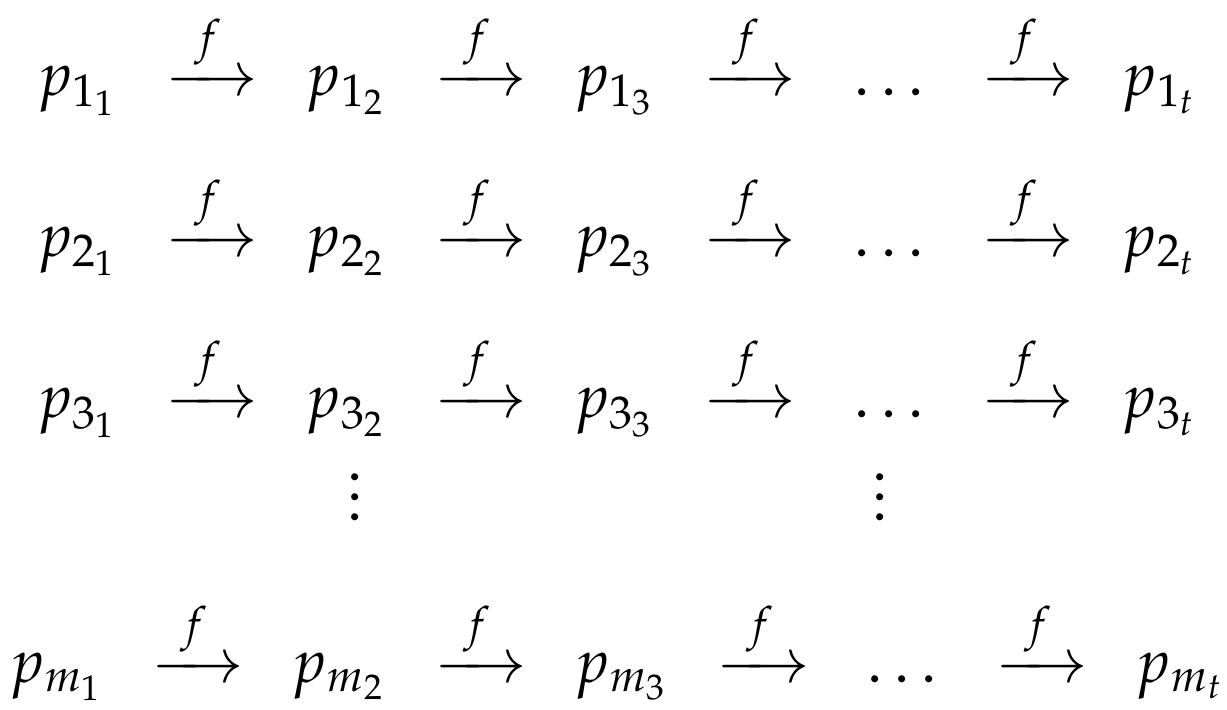
\includegraphics[scale=0.25]{tabla_2}
%\end{frame}
%
%\begin{frame}{TMTO}
%	Se guardan únicamente la primera y última entradas de cada fila.
%	El intercambio tiempo-memoria depende de las dimensiones escogidas para la tabla:
%	\begin{itemize}
%			
%		\item \textbf{Mayor número de filas}: Más tiempo necesario en la generación de la tabla, menos tiempo requerido en la búsqueda
%
%		\item \textbf{Mayor número de columnas}: Menor tiempo empleado en la construcción de la tabla, mayor tiempo necesario para la búsqueda.
%
%	\end{itemize}
%\end{frame}

\section{El ataque del arco iris}

\begin{frame}{Proceso}
	Obtener un mensaje de entrada $p$.\\
	~\\
	Generar su valor resumen $h = H(p)$.\\
	~\\
	Reconstruir el valor resumen $h$ en un mensaje de entrada válido, según el contexto.
\end{frame}

\begin{frame}{Función de reconstrucción}
	Toma como entrada un valor resumen y lo reconstruye en un mensaje válido según el contexto de la implementación.\\
	~\\
	\begin{center}
		$R(h) = p'$
	\end{center}
\end{frame}

\begin{frame}{Tablas del arco iris}

	\centering
	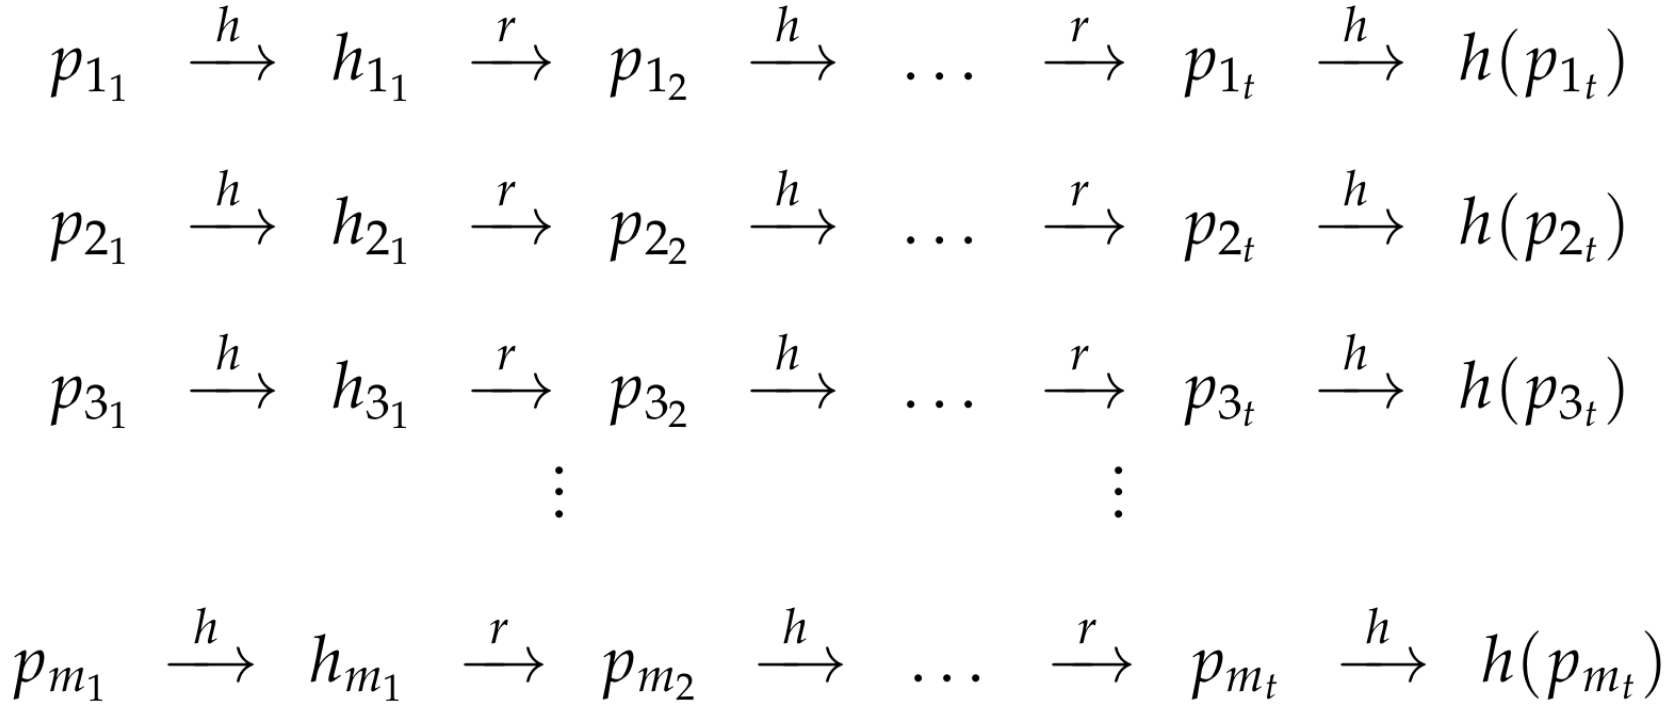
\includegraphics[scale=0.2]{rainbow_2.png}\\
	~\\
	Almacenar el mensaje inicial y el resumen final de cada fila\\

\end{frame}

\begin{frame}{Búsqueda de colisiones con una tabla del arco iris}
	Teniendo $\{p_{1_1}, h(p_{1_t})\}, \{p_{2_1}, h(p_{2_t})\}, \{p_{3_1}, h(p_{3_t})\}, \dots, \{p_{m_1}, h(p_{m_t})\}$\\
	~\\
	\pause
	\begin{enumerate}

		\item Comprobar las últimas entradas de la tabla. Detener la búsqueda con éxito si se encuentra la colisión en una de ellas.
		\pause
		\item Aplicar la función de reconstrucción seguida de la función resumen desde las últimas entradas
		\pause
	\item Repetir $t$ veces por cada fila hasta encontrar (o no) la colisión.

	\end{enumerate}
\end{frame}

\section{Estudio experimental}

\begin{frame}{Implementación desarrollada}
	\pause
	\textbf{Objetivo}: adivinar las contraseñas de acceso a un sistema operativo.\\
	~\\
	\pause
	\textbf{Dominio de colisiones}: contraseñas de seis dígitos, desde '000000' hasta '999999'.\\
	~\\
	\pause
	\textbf{Función resumen atacada}: CRC-32, la cual genera valores resumen de 32 bits de longitud.
\end{frame}

\begin{frame}{Función de reconstrucción \textbf{R1}}
	\centering
	$p = $~'112233' $\xrightarrow{CRC-32}~~ h = $~'3570\underline{655599}'~~$\xrightarrow{\textbf{R1}}~~ r = $~'655599'
\end{frame}

\begin{frame}
	\centering
	\def\arraystretch{1.5}
\begin{table}[H]
    \LARGE
    \centering
    \resizebox{\textwidth}{!}{\begin{tabular}{|c|r|c|c|c|c|c|c|c|c|c|c|c|c|c|}
        \hline
        \multirow{13}{*}{$t$} & 1 & & & & & & & & & & & & & \textcolor{g}{100\%} \\ \cline{2-15}
        & 2 & & & & & & & & & & & & \textcolor{b}{91.9\%} & \\ \cline{2-15}
        & 4 & & & & & & & & & & & \textcolor{b}{90.6\%} & & \\ \cline{2-15}
        & 5 & & & & & & & & & & \textcolor{b}{90.6\%} & & & \\ \cline{2-15}
        & 10 & & & & & & & & & \textcolor{g}{95.2\%} & & & & \\ \cline{2-15}
        & 20 & & & & & & & & \textcolor{g}{96.1\%} & & & & & \\ \cline{2-15}
        & 40 & & & & & & & \textcolor{g}{97.1\%} & & & & & & \\ \cline{2-15}
        & 50 & & & & & & \textcolor{g}{97.4\%} &  & \textcolor{g}{99.3\%} & \textcolor{g}{99.6\%} & & \textcolor{g}{99.6\%} & \textcolor{g}{100\%} & \textcolor{g}{100\%} \\ \cline{2-15}
        & 100 & & & & & \textcolor{g}{96.4\%} & \textcolor{g}{98.0\%} & \textcolor{g}{98.4\%} & \textcolor{g}{99.0\%} & \textcolor{g}{99.8\%} & & \textcolor{g}{100\%} & \textcolor{g}{100\%} & \textcolor{g}{100\%} \\ \cline{2-15}
        & 200 & & & & \textcolor{g}{95.2\%} & & & & & & & & & \\ \cline{2-15}
        & 400 & & & \textcolor{b}{91.8\%} & & & & & & & & & & \\ \cline{2-15}
        & 500 & & \textcolor{y}{84.1\%} & & & & & & & & & & & \\ \cline{2-15}
        & 1000 & \textcolor{r}{63.5\%} & & & & & & & & & & & & \\ \cline{2-15}
        & & 1000 & 2000 & 2500 & 5000 & 10000 & 20000 & 25000 & 50000 & 100000 & 200000 & 250000 & 500000 & 1000000 \\ \hline
        & & \multicolumn{13}{c|}{$m$} \\ \hline
    \end{tabular}}
    \caption{Porcentajes de éxito para las tablas empleando \textbf{R1}}
    \label{resR1}
\end{table}

\end{frame}

\begin{frame}{Función de reconstrucción \textbf{R2}}
	\centering
	$p = $~'112233' $\xrightarrow{CRC-32}~~ h_d = $~'3570655\underline{599}', $h_h = $~'\cancel{D4}D3E16F'~~$\xrightarrow{\textbf{R2}}$\\
	~\\
	~~$\xrightarrow{\textbf{R2}}~~ r = $'939165'
\end{frame}

\begin{frame}
	\def\arraystretch{1.5}
\begin{table}[H]
    \LARGE
    \centering
    \resizebox{\textwidth}{!}{\begin{tabular}{|c|r|c|c|c|c|c|c|c|c|c|c|c|c|c|}
        \hline
        \multirow{13}{*}{$t$} & 1 & & & & & & & & & & & & & \textcolor{g}{100\%} \\ \cline{2-15}
        & 2 & & & & & & & & & & & & \textcolor{b}{91.1\%} & \\ \cline{2-15}
        & 4 & & & & & & & & & & & \textcolor{b}{89.4\%} & & \\ \cline{2-15}
        & 5 & & & & & & & & & & \textcolor{b}{88.8\%} & & & \\ \cline{2-15}
        & 10 & & & & & & & & & \textcolor{b}{93.0\%} & & & & \\ \cline{2-15}
        & 20 & & & & & & & & \textcolor{g}{95.5\%} & & & & & \\ \cline{2-15}
        & 40 & & & & & & & \textcolor{g}{97.1\%} & & & & & & \\ \cline{2-15}
        & 50 & & & & & & \textcolor{g}{97.1\%} &  & \textcolor{g}{98.8\%} & \textcolor{g}{99.7\%} & & \textcolor{g}{100\%} & \textcolor{g}{100\%} & \textcolor{g}{100\%} \\ \cline{2-15}
        & 100 & & & & & \textcolor{g}{97.1\%} & \textcolor{g}{98.8\%} & \textcolor{g}{99.2\%} & \textcolor{g}{99.6\%} & \textcolor{g}{99.9\%} & & \textcolor{g}{99.9\%} & \textcolor{g}{99.9\%} & \textcolor{g}{100\%} \\ \cline{2-15}
        & 200 & & & & \textcolor{b}{94.3\%} & & & & & & & & & \\ \cline{2-15}
        & 400 & & & \textcolor{y}{82.1\%} & & & & & & & & & & \\ \cline{2-15}
        & 500 & & \textcolor{y}{74.9\%} & & & & & & & & & & & \\ \cline{2-15}
        & 1000 & \textcolor{r}{57.1\%} & & & & & & & & & & & & \\ \cline{2-15}
        & & 1000 & 2000 & 2500 & 5000 & 10000 & 20000 & 25000 & 50000 & 100000 & 200000 & 250000 & 500000 & 1000000 \\ \hline
        & & \multicolumn{13}{c|}{$m$} \\ \hline
    \end{tabular}}
    \caption{Porcentajes de éxito para las tablas empleando \textbf{R2}}
    \label{resR2}
\end{table}

\end{frame}

\begin{frame}
	\centering
	\def\arraystretch{1.5}
\begin{table}[H]
    \LARGE
    \centering
    \resizebox{\textwidth}{!}{\begin{tabular}{|c|r|c|c|c|c|c|c|c|c|c|c|c|c|c|}
        \hline
        \multirow{13}{*}{$t$} & 1 & & & & & & & & & & & & & \textcolor{g}{100\%} \\ \cline{2-15}
        & 2 & & & & & & & & & & & & \textcolor{b}{91.9\%} & \\ \cline{2-15}
        & 4 & & & & & & & & & & & \textcolor{b}{90.6\%} & & \\ \cline{2-15}
        & 5 & & & & & & & & & & \textcolor{b}{90.6\%} & & & \\ \cline{2-15}
        & 10 & & & & & & & & & \textcolor{g}{95.2\%} & & & & \\ \cline{2-15}
        & 20 & & & & & & & & \textcolor{g}{96.1\%} & & & & & \\ \cline{2-15}
        & 40 & & & & & & & \textcolor{g}{97.1\%} & & & & & & \\ \cline{2-15}
        & 50 & & & & & & \textcolor{g}{97.4\%} &  & \textcolor{g}{99.3\%} & \textcolor{g}{99.6\%} & & \textcolor{g}{99.6\%} & \textcolor{g}{100\%} & \textcolor{g}{100\%} \\ \cline{2-15}
        & 100 & & & & & \textcolor{g}{96.4\%} & \textcolor{g}{98.0\%} & \textcolor{g}{98.4\%} & \textcolor{g}{99.0\%} & \textcolor{g}{99.8\%} & & \textcolor{g}{100\%} & \textcolor{g}{100\%} & \textcolor{g}{100\%} \\ \cline{2-15}
        & 200 & & & & \textcolor{g}{95.2\%} & & & & & & & & & \\ \cline{2-15}
        & 400 & & & \textcolor{b}{91.8\%} & & & & & & & & & & \\ \cline{2-15}
        & 500 & & \textcolor{y}{84.1\%} & & & & & & & & & & & \\ \cline{2-15}
        & 1000 & \textcolor{r}{63.5\%} & & & & & & & & & & & & \\ \cline{2-15}
        & & 1000 & 2000 & 2500 & 5000 & 10000 & 20000 & 25000 & 50000 & 100000 & 200000 & 250000 & 500000 & 1000000 \\ \hline
        & & \multicolumn{13}{c|}{$m$} \\ \hline
    \end{tabular}}
    \caption{Porcentajes de éxito para las tablas empleando \textbf{R1}}
    \label{resR1_2}
\end{table}
\end{frame}

\begin{frame}{Combinando funciones de reconstrucción}
	\framesubtitle{Alternancia de funciones de reconstrucción}
	\centering
	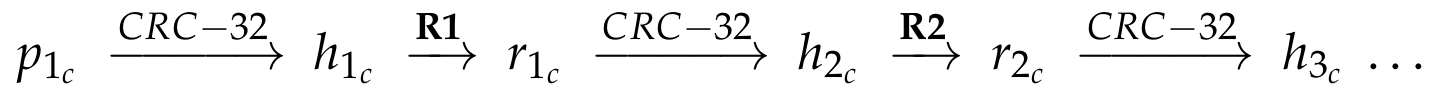
\includegraphics[scale=0.2]{filaR1R2}
\end{frame}

\begin{frame}
	\def\arraystretch{1.5}
\begin{table}[H]
    \LARGE
    \centering
    \resizebox{\textwidth}{!}{\begin{tabular}{|c|r|c|c|c|c|c|c|c|c|c|c|c|c|c|}
        \hline
        \multirow{13}{*}{$t$} & 1 & & & & & & & & & & & & & \textcolor{g}{100\%} \\ \cline{2-15}
        & 2 & & & & & & & & & & & & \textcolor{g}{97.0\%} & \\ \cline{2-15}
        & 4 & & & & & & & & & & & \textcolor{g}{96.2\%} & & \\ \cline{2-15}
        & 5 & & & & & & & & & & \textcolor{g}{97.0\%} & & & \\ \cline{2-15}
        & 10 & & & & & & & & & \textcolor{g}{98.3\%} & & & & \\ \cline{2-15}
        & 20 & & & & & & & & \textcolor{g}{99.5\%} & & & & & \\ \cline{2-15}
        & 40 & & & & & & & \textcolor{g}{99.7\%} & & & & & & \\ \cline{2-15}
        & 50 & & & & & & \textcolor{g}{99.6\%} &  & \textcolor{g}{100\%} & \textcolor{g}{100\%} & & \textcolor{g}{100\%} & \textcolor{g}{100\%} & \textcolor{g}{100\%} \\ \cline{2-15}
        & 100 & & & & & \textcolor{g}{99.9\%} & \textcolor{g}{99.9\%} & \textcolor{g}{99.9\%} & \textcolor{g}{100\%} & \textcolor{g}{100\%} & & \textcolor{g}{100\%} & \textcolor{g}{100\%} & \textcolor{g}{100\%} \\ \cline{2-15}
        & 200 & & & & \textcolor{g}{99.9\%} & & & & & & & & & \\ \cline{2-15}
        & 400 & & & \textcolor{g}{98.1\%} & & & & & & & & & & \\ \cline{2-15}
        & 500 & & \textcolor{g}{95.4\%} & & & & & & & & & & & \\ \cline{2-15}
        & 1000 & \textcolor{r}{63.1\%} & & & & & & & & & & & & \\ \cline{2-15}
        & & 1000 & 2000 & 2500 & 5000 & 10000 & 20000 & 25000 & 50000 & 100000 & 200000 & 250000 & 500000 & 1000000 \\ \hline
        & & \multicolumn{13}{c|}{$m$} \\ \hline
    \end{tabular}}
    \caption{Porcentajes de éxito para las tablas empleando la alternancia de las funciones de reconstrucción}
    \label{resR1R2}
\end{table}

\end{frame}

\begin{frame}{Combinando funciones de reconstrucción}
	\framesubtitle{Combinación mediante un patrón}
	\centering
	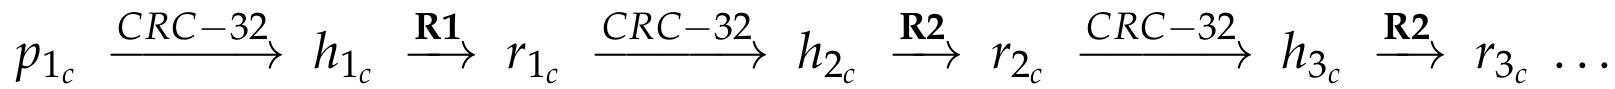
\includegraphics[scale=0.2]{filapp}
\end{frame}

\begin{frame}
	\def\arraystretch{1.5}
\begin{table}[H]
    \LARGE
    \centering
    \resizebox{\textwidth}{!}{\begin{tabular}{|c|r|c|c|c|c|c|c|c|c|c|c|c|c|c|}
        \hline
        \multirow{13}{*}{$t$} & 1 & & & & & & & & & & & & & \textcolor{g}{100\%} \\ \cline{2-15}
        & 2 & & & & & & & & & & & & \textcolor{g}{98.1\%} & \\ \cline{2-15}
        & 4 & & & & & & & & & & & \textcolor{g}{98.9\%} & & \\ \cline{2-15}
        & 5 & & & & & & & & & & \textcolor{g}{99.4\%} & & & \\ \cline{2-15}
        & 10 & & & & & & & & & \textcolor{g}{99.8\%} & & & & \\ \cline{2-15}
        & 20 & & & & & & & & \textcolor{g}{100\%} & & & & & \\ \cline{2-15}
        & 40 & & & & & & & \textcolor{g}{100\%} & & & & & & \\ \cline{2-15}
        & 50 & & & & & & \textcolor{g}{100\%} &  & \textcolor{g}{100\%} & \textcolor{g}{100\%} & & \textcolor{g}{100\%} & \textcolor{g}{100\%} & \textcolor{g}{100\%} \\ \cline{2-15}
        & 100 & & & & & \textcolor{g}{100\%} & \textcolor{g}{100\%} & \textcolor{g}{100\%} & \textcolor{g}{100\%} & \textcolor{g}{100\%} & & \textcolor{g}{100\%} & \textcolor{g}{100\%} & \textcolor{g}{100\%} \\ \cline{2-15}
        & 200 & & & & \textcolor{g}{100\%} & & & & & & & & & \\ \cline{2-15}
        & 400 & & & \textcolor{g}{99.5\%} & & & & & & & & & & \\ \cline{2-15}
        & 500 & & \textcolor{g}{99.3\%} & & & & & & & & & & & \\ \cline{2-15}
        & 1000 & \textcolor{y}{80.5\%} & & & & & & & & & & & & \\ \cline{2-15}
        & & 1000 & 2000 & 2500 & 5000 & 10000 & 20000 & 25000 & 50000 & 100000 & 200000 & 250000 & 500000 & 1000000 \\ \hline
        & & \multicolumn{13}{c|}{$m$} \\ \hline
    \end{tabular}}
    \caption{Porcentajes de éxito para las tablas empleando el patrón reducido}
    \label{respp}
\end{table}
test
\end{frame}

\begin{frame}{Combinando funciones de reconstrucción}
	\framesubtitle{Un patrón más extenso}
	\centering
	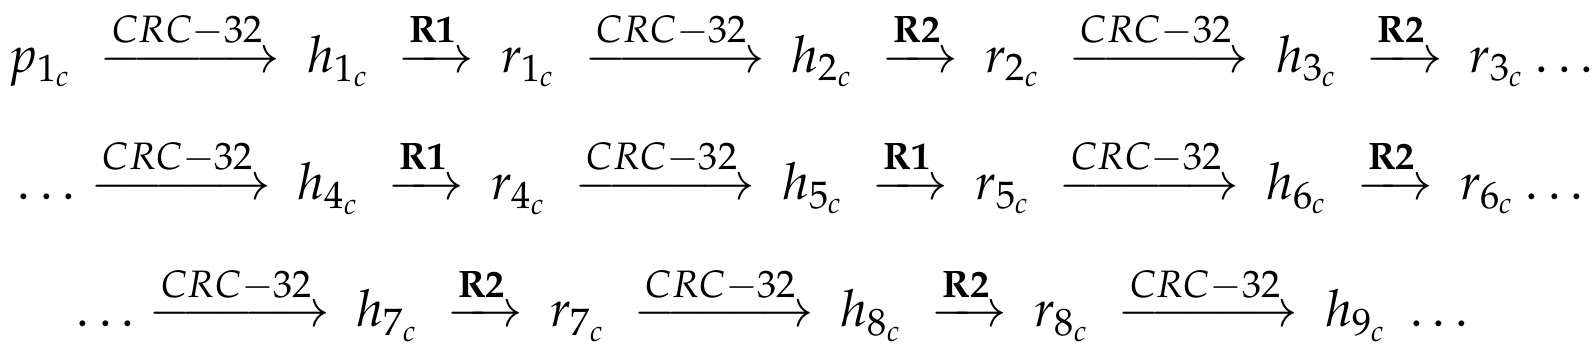
\includegraphics[scale=0.2]{filaPG}
\end{frame}

\begin{frame}
	\def\arraystretch{1.5}
\begin{table}[H]
    \LARGE
    \centering
    \resizebox{\textwidth}{!}{\begin{tabular}{|c|r|c|c|c|c|c|c|c|c|c|c|c|c|c|}
        \hline
        \multirow{13}{*}{$t$} & 1 & & & & & & & & & & & & & \textcolor{g}{100\%} \\ \cline{2-15}
        & 2 & & & & & & & & & & & & \textcolor{g}{98.5\%} & \\ \cline{2-15}
        & 4 & & & & & & & & & & & \textcolor{g}{99.9\%} & & \\ \cline{2-15}
        & 5 & & & & & & & & & & \textcolor{g}{100\%} & & & \\ \cline{2-15}
        & 10 & & & & & & & & & \textcolor{g}{100\%} & & & & \\ \cline{2-15}
        & 20 & & & & & & & & \textcolor{g}{100\%} & & & & & \\ \cline{2-15}
        & 40 & & & & & & & \textcolor{g}{100\%} & & & & & & \\ \cline{2-15}
        & 50 & & & & & & \textcolor{g}{100\%} &  & \textcolor{g}{100\%} & \textcolor{g}{100\%} & & \textcolor{g}{100\%} & \textcolor{g}{100\%} & \textcolor{g}{100\%} \\ \cline{2-15}
        & 100 & & & & & \textcolor{g}{100\%} & \textcolor{g}{100\%} & \textcolor{g}{100\%} & \textcolor{g}{100\%} & \textcolor{g}{100\%} & & \textcolor{g}{100\%} & \textcolor{g}{100\%} & \textcolor{g}{100\%} \\ \cline{2-15}
        & 200 & & & & \textcolor{g}{100\%} & & & & & & & & & \\ \cline{2-15}
        & 400 & & & \textcolor{g}{100\%} & & & & & & & & & & \\ \cline{2-15}
        & 500 & & \textcolor{g}{100\%} & & & & & & & & & & & \\ \cline{2-15}
        & 1000 & \textcolor{r}{63.0\%} & & & & & & & & & & & & \\ \cline{2-15}
        & & 1000 & 2000 & 2500 & 5000 & 10000 & 20000 & 25000 & 50000 & 100000 & 200000 & 250000 & 500000 & 1000000 \\ \hline
        & & \multicolumn{13}{c|}{$m$} \\ \hline
    \end{tabular}}
    \caption{Porcentajes de éxito para las tablas empleando el patrón extenso}
    \label{resPG}
\end{table}

\end{frame}

%\begin{frame}
%
%\def\arraystretch{1.5}
%\begin{table}%[H]
%    \centering
%    \resizebox{\textwidth}{!}{\begin{tabular}{|c|r|c|c|c|c|c|c|c|c|c|}
%        \hline
%        \multirow{6}{*}{$t$} & 50 & \textcolor{g}{0.80\%} & \textcolor{g}{1.80\%} & \textcolor{g}{2.40\%} & \textcolor{g}{2.60\%} & \textcolor{g}{4.27\%} & \textcolor{g}{5.15\%} & \textcolor{g}{5.80\%} & \textcolor{g}{10.16\%} & \textcolor{g}{19.08\%} \\ \cline{2-11}
%        & 100 & \textcolor{g}{2.00\%} & \textcolor{g}{2.60\%} & \textcolor{g}{4.00\%} & \textcolor{g}{5.00\%} & \textcolor{g}{7.47\%} & \textcolor{g}{9.55\%} & \textcolor{g}{10.76\%} & \textcolor{g}{18.96\%} & \textcolor{b}{32.75\%} \\ \cline{2-11}
%        & 200 & \textcolor{g}{3.60\%} & \textcolor{g}{4.60\%} & \textcolor{g}{6.80\%} & \textcolor{g}{8.90\%} & \textcolor{g}{13.00\%} & \textcolor{g}{16.00\%} & \textcolor{g}{17.92\%} & \textcolor{b}{30.60\%} & \textcolor{b}{47.18\%} \\ \cline{2-11}
%        & 400 & \textcolor{g}{5.20\%} & \textcolor{g}{8.40\%} & \textcolor{g}{13.07\%} & \textcolor{g}{16.50\%} & \textcolor{g}{23.47\%} & \textcolor{b}{28.55\%} & \textcolor{b}{31.96\%} & \textcolor{b}{48.74\%} & \textcolor{y}{65.83\%} \\ \cline{2-11}
%        & 500 & \textcolor{g}{6.00\%} & \textcolor{g}{10.00\%} & \textcolor{g}{15.20\%} & \textcolor{g}{19.40\%} & \textcolor{b}{27.00\%} & \textcolor{b}{32.55\%} & \textcolor{b}{36.68\%} & \textcolor{y}{54.74\%} & \textcolor{r}{71.14\%} \\ \cline{2-11}
%		& 1000 & \textcolor{g}{\phantom{0}9.20\%} & \textcolor{g}{13.60\%} & \textcolor{g}{18.93\%} & \textcolor{g}{24.00\%} & \textcolor{b}{33.20\%} & \textcolor{b}{40.35\%} & \textcolor{b}{45.68\%} & \textcolor{y}{65.02\%} & \textcolor{r}{79.64\%} \\ \hline
%        & & 250 & 500 & 750 & 1000 & 1500 & 2000 & 2500 & 5000 & 10000 \\ \hline
%        & & \multicolumn{9}{c|}{$m$} \\ \hline
%    \end{tabular}}
%    \caption{Porcentajes de colisiones para las tablas empleando únicamente la función de reconstrucción \textbf{R1}}
%    \label{colR1}
%\end{table}
%	
%\end{frame}
%
%\begin{frame}
%
%	\def\arraystretch{1.5}
%\begin{table}%[H]
%    \centering
%    \resizebox{\textwidth}{!}{\begin{tabular}{|c|r|c|c|c|c|c|c|c|c|c|}
%        \hline
%        \multirow{6}{*}{$t$} & 50 & \textcolor{g}{0.00\%} & \textcolor{g}{1.60\%} & \textcolor{g}{2.00\%} & \textcolor{g}{2.60\%} & \textcolor{g}{4.20\%} & \textcolor{g}{5.70\%} & \textcolor{g}{6.64\%} & \textcolor{g}{12.52\%} & \textcolor{g}{22.60\%} \\ \cline{2-11}
%        & 100 & \textcolor{g}{0.40\%} & \textcolor{g}{2.60\%} & \textcolor{g}{4.27\%} & \textcolor{g}{5.50\%} & \textcolor{g}{8.13\%} & \textcolor{g}{10.15\%} & \textcolor{g}{12.32\%} & \textcolor{g}{22.50\%} & \textcolor{b}{36.42\%} \\ \cline{2-11}
%        & 200 & \textcolor{g}{2.80\%} & \textcolor{g}{7.20\%} & \textcolor{g}{9.47\%} & \textcolor{g}{12.40\%} & \textcolor{g}{16.27\%} & \textcolor{g}{18.80\%} & \textcolor{g}{21.60\%} & \textcolor{b}{34.72\%} & \textcolor{y}{51.27\%} \\ \cline{2-11}
%        & 400 & \textcolor{g}{11.60\%} & \textcolor{g}{18.00\%} & \textcolor{g}{21.73\%} & \textcolor{b}{27.10\%} & \textcolor{b}{34.13\%} & \textcolor{b}{38.75\%} & \textcolor{b}{43.28\%} & \textcolor{y}{58.74\%} & \textcolor{r}{73.00\%} \\ \cline{2-11}
%        & 500 & \textcolor{g}{15.60\%} & \textcolor{g}{23.60\%} & \textcolor{b}{27.60\%} & \textcolor{b}{33.40\%} & \textcolor{b}{41.07\%} & \textcolor{b}{46.50\%} & \textcolor{y}{51.68\%} & \textcolor{y}{67.52\%} & \textcolor{r}{79.88\%} \\ \cline{2-11}
%        & 1000 & \textcolor{g}{18.00\%} & \textcolor{b}{28.80\%} & \textcolor{b}{35.87\%} & \textcolor{b}{42.80\%} & \textcolor{y}{53.67\%} & \textcolor{y}{60.95\%} & \textcolor{y}{66.76\%} & \textcolor{r}{81.62\%} & \textcolor{r}{90.47\%} \\ \hline
%        & & 250 & 500 & 750 & 1000 & 1500 & 2000 & 2500 & 5000 & 10000 \\ \hline
%        & & \multicolumn{9}{c|}{$m$} \\ \hline
%    \end{tabular}}
%    \caption{Porcentajes de colisiones para las tablas empleando únicamente la función de reconstrucción \textbf{R2}}
%    \label{colR2}
%\end{table}
%
%\end{frame}
%
%\begin{frame}
%
%	\def\arraystretch{1.5}
%\begin{table}%[H]
%    \centering
%    \resizebox{\textwidth}{!}{\begin{tabular}{|c|r|c|c|c|c|c|c|c|c|c|}
%        \hline
%        \multirow{6}{*}{$t$} & 50 & \textcolor{g}{0.80\%} & \textcolor{g}{1.00\%} & \textcolor{g}{1.73\%} & \textcolor{g}{2.30\%} & \textcolor{g}{3.93\%} & \textcolor{g}{5.30\%} & \textcolor{g}{6.32\%} & \textcolor{g}{11.48\%} & \textcolor{g}{20.74\%} \\ \cline{2-11}
%        & 100 & \textcolor{g}{0.80\%} & \textcolor{g}{1.60\%} & \textcolor{g}{3.07\%} & \textcolor{g}{4.30\%} & \textcolor{g}{6.80\%} & \textcolor{g}{8.80\%} & \textcolor{g}{10.96\%} & \textcolor{g}{19.48\%} & \textcolor{b}{33.78\%} \\ \cline{2-11}
%        & 200 & \textcolor{g}{2.00\%} & \textcolor{g}{4.80\%} & \textcolor{g}{6.67\%} & \textcolor{g}{8.30\%} & \textcolor{g}{12.60\%} & \textcolor{g}{16.65\%} & \textcolor{g}{20.00\%} & \textcolor{b}{32.16\%} & \textcolor{b}{49.08\%} \\ \cline{2-11}
%        & 400 & \textcolor{g}{2.40\%} & \textcolor{g}{9.00\%} & \textcolor{g}{12.80\%} & \textcolor{g}{17.80\%} & \textcolor{g}{23.00\%} & \textcolor{b}{29.05\%} & \textcolor{b}{33.24\%} & \textcolor{b}{47.44\%} & \textcolor{y}{63.71\%} \\ \cline{2-11}
%        & 500 & \textcolor{g}{3.20\%} & \textcolor{g}{11.00\%} & \textcolor{g}{16.13\%} & \textcolor{g}{21.80\%} & \textcolor{b}{27.33\%} & \textcolor{b}{33.60\%} & \textcolor{b}{38.24\%} & \textcolor{y}{52.96\%} & \textcolor{y}{68.54\%} \\ \cline{2-11}
%		& 1000 & \textcolor{g}{\phantom{0}9.60\%} & \textcolor{g}{21.40\%} & \textcolor{b}{29.20\%} & \textcolor{b}{36.90\%} & \textcolor{b}{46.00\%} & \textcolor{y}{53.40\%} & \textcolor{y}{59.24\%} & \textcolor{r}{74.32\%} & \textcolor{r}{85.00\%} \\ \hline
%        & & 250 & 500 & 750 & 1000 & 1500 & 2000 & 2500 & 5000 & 10000 \\ \hline
%        & & \multicolumn{9}{c|}{$m$} \\ \hline
%    \end{tabular}}
%    \caption{Porcentajes de colisiones para las tablas empleando la alternancia de las funciones de reconstrucción}
%    \label{colR1R2}
%\end{table}
%
%\end{frame}
%
%\begin{frame}
%
%\def\arraystretch{1.5}
%\begin{table}[H]
%    \centering
%    \resizebox{\textwidth}{!}{\begin{tabular}{|c|r|c|c|c|c|c|c|c|c|c|}
%        \hline
%        \multirow{6}{*}{$t$} & 50 & \textcolor{g}{0.80\%} & \textcolor{g}{0.60\%} & \textcolor{g}{0.80\%} & \textcolor{g}{1.10\%} & \textcolor{g}{1.73\%} & \textcolor{g}{2.00\%} & \textcolor{g}{2.68\%} & \textcolor{g}{4.86\%} & \textcolor{g}{9.30\%} \\ \cline{2-11}
%        & 100 & \textcolor{g}{1.20\%} & \textcolor{g}{1.40\%} & \textcolor{g}{2.13\%} & \textcolor{g}{2.70\%} & \textcolor{g}{3.53\%} & \textcolor{g}{4.35\%} & \textcolor{g}{5.56\%} & \textcolor{g}{9.08\%} & \textcolor{g}{16.16\%} \\ \cline{2-11}
%        & 200 & \textcolor{g}{1.60\%} & \textcolor{g}{2.00\%} & \textcolor{g}{2.80\%} & \textcolor{g}{3.80\%} & \textcolor{g}{5.40\%} & \textcolor{g}{6.75\%} & \textcolor{g}{8.44\%} & \textcolor{g}{14.32\%} & \textcolor{b}{25.46\%} \\ \cline{2-11}
%        & 400 & \textcolor{g}{2.00\%} & \textcolor{g}{4.00\%} & \textcolor{g}{5.07\%} & \textcolor{g}{6.70\%} & \textcolor{g}{9.87\%} & \textcolor{g}{12.70\%} & \textcolor{g}{15.44\%} & \textcolor{g}{24.70\%} & \textcolor{b}{39.64\%} \\ \cline{2-11}
%        & 500 & \textcolor{g}{1.60\%} & \textcolor{g}{3.80\%} & \textcolor{g}{5.73\%} & \textcolor{g}{7.40\%} & \textcolor{g}{11.47\%} & \textcolor{g}{14.65\%} & \textcolor{g}{17.80\%} & \textcolor{b}{29.54\%} & \textcolor{b}{45.17\%} \\ \cline{2-11}
%		& 1000 & \textcolor{g}{\phantom{0}5.60\%} & \textcolor{g}{11.80\%} & \textcolor{g}{16.13\%} & \textcolor{g}{18.90\%} & \textcolor{b}{25.87\%} & \textcolor{b}{30.75\%} & \textcolor{b}{35.08\%} & \textcolor{y}{51.08\%} & \textcolor{y}{67.09\%} \\ \hline
%        & & 250 & 500 & 750 & 1000 & 1500 & 2000 & 2500 & 5000 & 10000 \\ \hline
%        & & \multicolumn{9}{c|}{$m$} \\ \hline
%    \end{tabular}}
%    \caption{Porcentajes de colisiones para las tablas empleando el patrón reducido de funciones de reconstrucción}
%    \label{colpp}
%\end{table}
%
%\end{frame}
%
%\begin{frame}
%
%\def\arraystretch{1.5}
%\begin{table}[H]
%    \centering
%    \resizebox{\textwidth}{!}{\begin{tabular}{|c|r|c|c|c|c|c|c|c|c|c|}
%        \hline
%        \multirow{6}{*}{$t$} & 50 & \textcolor{g}{0.00\%} & \textcolor{g}{0.40\%} & \textcolor{g}{0.67\%} & \textcolor{g}{0.80\%} & \textcolor{g}{1.27\%} & \textcolor{g}{1.70\%} & \textcolor{g}{2.04\%} & \textcolor{g}{3.18\%} & \textcolor{g}{6.70\%} \\ \cline{2-11}
%        & 100 & \textcolor{g}{1.20\%} & \textcolor{g}{1.20\%} & \textcolor{g}{1.60\%} & \textcolor{g}{2.30\%} & \textcolor{g}{3.93\%} & \textcolor{g}{4.80\%} & \textcolor{g}{5.60\%} & \textcolor{g}{11.20\%} & \textcolor{g}{20.63\%} \\ \cline{2-11}
%        & 200 & \textcolor{g}{2.40\%} & \textcolor{g}{4.60\%} & \textcolor{g}{7.87\%} & \textcolor{g}{9.50\%} & \textcolor{g}{14.67\%} & \textcolor{g}{17.55\%} & \textcolor{g}{20.28\%} & \textcolor{b}{33.68\%} & \textcolor{y}{50.76\%} \\ \cline{2-11}
%        & 400 & \textcolor{g}{4.00\%} & \textcolor{g}{8.00\%} & \textcolor{g}{12.80\%} & \textcolor{g}{16.50\%} & \textcolor{g}{23.53\%} & \textcolor{b}{28.25\%} & \textcolor{b}{32.44\%} & \textcolor{b}{48.94\%} & \textcolor{y}{65.97\%} \\ \cline{2-11}
%        & 500 & \textcolor{g}{3.60\%} & \textcolor{g}{4.60\%} & \textcolor{g}{7.87\%} & \textcolor{g}{10.20\%} & \textcolor{g}{15.73\%} & \textcolor{g}{18.80\%} & \textcolor{g}{22.12\%} & \textcolor{b}{36.64\%} & \textcolor{y}{54.28\%} \\ \cline{2-11}
%        & 1000 & \textcolor{g}{10.40\%} & \textcolor{g}{21.80\%} & \textcolor{b}{30.80\%} & \textcolor{b}{36.80\%} & \textcolor{b}{45.33\%} & \textcolor{y}{51.30\%} & \textcolor{y}{55.88\%} & \textcolor{r}{70.64\%} & \textcolor{r}{82.47\%} \\ \hline
%        & & 250 & 500 & 750 & 1000 & 1500 & 2000 & 2500 & 5000 & 10000 \\ \hline
%        & & \multicolumn{9}{c|}{$m$} \\ \hline
%    \end{tabular}}
%    \caption{Porcentajes de colisiones para las tablas empleando el patrón extenso de funciones de reconstrucción}
%    \label{colPG}
%\end{table}
%
%\end{frame}

\begin{frame}

\def\arraystretch{1.5}
\begin{table}[H]
    \centering
	\resizebox{\textwidth}{!}{\begin{tabular}{|c|r|c|c|c|c|c|c|c|c|c|}
        \hline
		\multirow{6}{*}{$t$} & 50 & \textcolor{r}{14.6\%} & \textcolor{r}{27.9\%} & \textcolor{r}{39.0\%} & \textcolor{r}{46.6\%} & \textcolor{r}{59.4\%} & \textcolor{r}{67.8\%} & \textcolor{y}{73.8\%} & \textcolor{b}{87.4\%} & \textcolor{b}{94.7\%} \\ \cline{2-10} \Cline{11-11}
		& 100 & \textcolor{r}{22.1\%} & \textcolor{r}{41.9\%} & \textcolor{r}{55.8\%} & \textcolor{r}{65.8\%} & \textcolor{y}{77.2\%} & \textcolor{y}{81.6\%} & \textcolor{b}{85.9\%} & \textcolor{b}{92.3\%} & \Thickvrulel{\textcolor{g}{96.4\%}} \\ \cline{2-9} \Cline{10-10} \cline{11-11}
		& 200 & \textcolor{r}{24.0\%} & \textcolor{r}{46.2\%} & \textcolor{r}{61.2\%} & \textcolor{y}{71.3\%} & \textcolor{y}{81.6\%} & \textcolor{b}{87.7\%} & \textcolor{b}{91.0\%} & \Thickvrulel{\textcolor{g}{95.2\%}} & \textcolor{g}{97.7\%} \\ \cline{2-11}
		& 400 & \textcolor{r}{23.7\%} & \textcolor{r}{45.0\%} & \textcolor{r}{60.5\%} & \textcolor{r}{69.9\%} & \textcolor{y}{82.1\%} & \textcolor{b}{88.5\%} & \textcolor{b}{91.8\%} & \Thickvrulel{\textcolor{g}{96.0\%}} & \textcolor{g}{98.3\%} \\ \cline{2-9} \Cline{10-10} \cline{11-11}
		& 500 & \textcolor{r}{23.5\%} & \textcolor{r}{44.3\%} & \textcolor{r}{58.2\%} & \textcolor{r}{67.0\%} & \textcolor{y}{78.3\%} & \textcolor{y}{84.1\%} & \textcolor{b}{87.9\%} & \textcolor{b}{94.6\%} & \Thickvrulel{\textcolor{g}{97.9\%}} \\ \cline{2-10} \Cline{11-11}
        & 1000 & \textcolor{r}{22.7\%} & \textcolor{r}{42.4\%} & \textcolor{r}{55.1\%} & \textcolor{r}{63.5\%} & \textcolor{y}{72.7\%} & \textcolor{y}{77.6\%} & \textcolor{y}{80.7\%} & \textcolor{b}{86.2\%} & \textcolor{b}{89.3\%} \\ \hline
        & & 250 & 500 & 750 & 1000 & 1500 & 2000 & 2500 & 5000 & 10000 \\ \hline
        & & \multicolumn{9}{c|}{$m$} \\ \hline
	\end{tabular}}
    \caption{Porcentajes de éxito para las tablas que emplean tan sólo la función de reconstrucción \textbf{R1}}
    \label{exR1}
\end{table}

\end{frame}

\begin{frame}

\def\arraystretch{1.5}
\begin{table}[H]
    \centering
    \resizebox{\textwidth}{!}{\begin{tabular}{|c|r|c|c|c|c|c|c|c|c|c|}
        \hline
		\multirow{6}{*}{$t$} & 50 & \textcolor{r}{15.9\%} & \textcolor{r}{29.7\%} & \textcolor{r}{40.2\%} & \textcolor{r}{48.8\%} & \textcolor{r}{61.2\%} & \textcolor{r}{69.7\%} & \textcolor{y}{76.0\%} & \textcolor{b}{88.6\%} & \textcolor{b}{94.4\%} \\ \cline{2-10} \Cline{11-11}
		& 100 & \textcolor{r}{22.2\%} & \textcolor{r}{41.7\%} & \textcolor{r}{56.2\%} & \textcolor{r}{66.2\%} & \textcolor{y}{76.9\%} & \textcolor{y}{82.8\%} & \textcolor{b}{87.0\%} & \textcolor{b}{93.4\%} & \Thickvrulel{\textcolor{g}{97.1\%}} \\ \cline{2-11}
		& 200 & \textcolor{r}{24.1\%} & \textcolor{r}{44.4\%} & \textcolor{r}{61.2\%} & \textcolor{y}{70.3\%} & \textcolor{y}{82.1\%} & \textcolor{b}{87.3\%} & \textcolor{b}{90.2\%} & \textcolor{b}{94.3\%} & \Thickvrulel{\textcolor{g}{97.4\%}} \\ \cline{2-10} \Cline{11-11}
        & 400 & \textcolor{r}{22.1\%} & \textcolor{r}{41.0\%} & \textcolor{r}{57.0\%} & \textcolor{r}{64.7\%} & \textcolor{y}{74.6\%} & \textcolor{y}{78.9\%} & \textcolor{y}{82.1\%} & \textcolor{b}{90.1\%} & \textcolor{b}{93.8\%} \\ \cline{2-11}
        & 500 & \textcolor{r}{21.1\%} & \textcolor{r}{38.2\%} & \textcolor{r}{53.1\%} & \textcolor{r}{60.8\%} & \textcolor{y}{69.3\%} & \textcolor{y}{74.9\%} & \textcolor{y}{77.6\%} & \textcolor{y}{81.9\%} & \textcolor{b}{85.3\%} \\ \cline{2-11}
        & 1000 & \textcolor{r}{20.5\%} & \textcolor{r}{35.6\%} & \textcolor{r}{48.0\%} & \textcolor{r}{57.1\%} & \textcolor{y}{69.4\%} & \textcolor{y}{73.8\%} & \textcolor{y}{76.1\%} & \textcolor{y}{79.3\%} & \textcolor{y}{79.6\%} \\ \hline
        & & 250 & 500 & 750 & 1000 & 1500 & 2000 & 2500 & 5000 & 10000 \\ \hline
        & & \multicolumn{9}{c|}{$m$} \\ \hline
    \end{tabular}}
    \caption{Porcentajes de éxito para las tablas que emplean tan sólo la función de reconstrucción \textbf{R2}}
    \label{exR2}
\end{table}

\end{frame}

\begin{frame}

\def\arraystretch{1.5}
\begin{table}[H]
    \centering
    \resizebox{\textwidth}{!}{\begin{tabular}{|c|r|c|c|c|c|c|c|c|c|c|}
		\cline{1-9} \Cline{10-11}
		\multirow{6}{*}{$t$} & 50 & \textcolor{r}{15.5\%} & \textcolor{r}{29.4\%} & \textcolor{r}{42.5\%} & \textcolor{r}{51.5\%} & \textcolor{r}{65.8\%} & \textcolor{y}{75.9\%} & \textcolor{y}{82.4\%} & \Thickvrulel{\textcolor{g}{96.1\%}} & \textcolor{g}{98.8\%} \\ \cline{2-8} \Cline{9-9} \cline{10-11}
		& 100 & \textcolor{r}{23.8\%} & \textcolor{r}{45.4\%} & \textcolor{r}{63.3\%} & \textcolor{y}{74.5\%} & \textcolor{b}{88.3\%} & \textcolor{b}{93.8\%} & \Thickvrulel{\textcolor{g}{96.2\%}} & \textcolor{g}{99.4\%} & \textcolor{g}{99.9\%} \\ \cline{2-7} \Cline{8-8} \cline{9-11}
		& 200 & \textcolor{r}{24.4\%} & \textcolor{r}{47.3\%} & \textcolor{r}{68.2\%} & \textcolor{y}{83.6\%} & \textcolor{b}{94.4\%} & \Thickvrulel{\textcolor{g}{97.2\%}} & \textcolor{g}{98.1\%} & \textcolor{g}{99.9\%} & \textcolor{g}{100\%} \\ \cline{2-11}
		& 400 & \textcolor{r}{24.4\%} & \textcolor{r}{45.3\%} & \textcolor{r}{64.1\%} & \textcolor{y}{77.3\%} & \textcolor{b}{92.6\%} & \Thickvrulel{\textcolor{g}{96.8\%}} & \textcolor{g}{98.1\%} & \textcolor{g}{99.8\%} & \textcolor{g}{100\%} \\ \cline{2-11}
		& 500 & \textcolor{r}{24.2\%} & \textcolor{r}{44.5\%} & \textcolor{r}{62.3\%} & \textcolor{y}{74.4\%} & \textcolor{b}{89.9\%} & \Thickvrulel{\textcolor{g}{95.4\%}} & \textcolor{g}{97.7\%} & \textcolor{g}{99.6\%} & \textcolor{g}{100\%} \\ \cline{2-7} \Cline{8-9} \cline{10-11}
		& 1000 & \textcolor{r}{22.6\%} & \textcolor{r}{39.3\%} & \textcolor{r}{53.1\%} & \textcolor{r}{63.1\%} & \textcolor{y}{77.3\%} & \textcolor{b}{85.9\%} & \textcolor{b}{89.9\%} & \Thickvrulel{\textcolor{g}{95.4\%}} & \textcolor{g}{97.9\%} \\ \cline{1-9} \Cline{10-11}
        & & 250 & 500 & 750 & 1000 & 1500 & 2000 & 2500 & 5000 & 10000 \\ \hline
        & & \multicolumn{9}{c|}{$m$} \\ \hline
    \end{tabular}}
    \caption{Porcentajes de éxito para las tablas que emplean la alternancia de funciones de reconstrucción}
    \label{exR1R2}
\end{table}

\end{frame}

\begin{frame}

\def\arraystretch{1.5}
\begin{table}[H]
    \centering
    \resizebox{\textwidth}{!}{\begin{tabular}{|c|r|c|c|c|c|c|c|c|c|c|}
		\cline{1-9} \Cline{10-11}
		\multirow{6}{*}{$t$} & 50 & \textcolor{r}{17.0\%} & \textcolor{r}{32.0\%} & \textcolor{r}{45.6\%} & \textcolor{r}{55.5\%} & \textcolor{y}{71.0\%} & \textcolor{y}{82.0\%} & \textcolor{b}{88.2\%} & \Thickvrulel{\textcolor{g}{98.0\%}} & \textcolor{g}{99.8\%} \\ \cline{2-7} \Cline{8-9} \cline{10-11}
		& 100 & \textcolor{r}{22.9\%} & \textcolor{r}{44.7\%} & \textcolor{r}{63.6\%} & \textcolor{y}{76.7\%} & \textcolor{b}{91.8\%} & \Thickvrulel{\textcolor{g}{96.5\%}} & \textcolor{g}{98.5\%} & \textcolor{g}{100\%} & \textcolor{g}{100\%} \\ \cline{2-6} \Cline{7-7} \cline{8-11}
		& 200 & \textcolor{r}{24.4\%} & \textcolor{r}{48.0\%} & \textcolor{r}{69.4\%} & \textcolor{b}{85.8\%} & \Thickvrulel{\textcolor{g}{97.3\%}} & \textcolor{g}{99.3\%} & \textcolor{g}{99.7\%} & \textcolor{g}{100\%} & \textcolor{g}{100\%} \\ \cline{2-11}
		& 400 & \textcolor{r}{24.5\%} & \textcolor{r}{47.8\%} & \textcolor{y}{70.9\%} & \textcolor{b}{88.0\%} & \Thickvrulel{\textcolor{g}{96.0\%}} & \textcolor{g}{99.0\%} & \textcolor{g}{99.5\%} & \textcolor{g}{99.9\%} & \textcolor{g}{100\%} \\ \cline{2-11}
		& 500 & \textcolor{r}{24.6\%} & \textcolor{r}{48.0\%} & \textcolor{y}{70.5\%} & \textcolor{b}{88.0\%} & \Thickvrulel{\textcolor{g}{97.2\%}} & \textcolor{g}{99.3\%} & \textcolor{g}{99.7\%} & \textcolor{g}{100\%} & \textcolor{g}{100\%} \\ \cline{2-11}
		& 1000 & \textcolor{r}{23.6\%} & \textcolor{r}{43.9\%} & \textcolor{r}{62.7\%} & \textcolor{y}{80.5\%} & \Thickvrulel{\textcolor{g}{95.6\%}} & \textcolor{g}{99.1\%} & \textcolor{g}{99.8\%} & \textcolor{g}{99.9\%} & \textcolor{g}{100\%} \\ \cline{1-6} \Cline{7-11}
        & & 250 & 500 & 750 & 1000 & 1500 & 2000 & 2500 & 5000 & 10000 \\ \hline
        & & \multicolumn{9}{c|}{$m$} \\ \hline
    \end{tabular}}
    \caption{Porcentajes de éxito para las tablas que emplean patrón reducido de funciones de reconstrucción}
    \label{expp}
\end{table}

\end{frame}

\begin{frame}

\def\arraystretch{1.5}
\begin{table}[H]
    \centering
    \resizebox{\textwidth}{!}{\begin{tabular}{|c|r|c|c|c|c|c|c|c|c|c|}
		\cline{1-9} \Cline{10-11}
		\multirow{6}{*}{$t$} & 50 & \textcolor{r}{18.9\%} & \textcolor{r}{36.2\%} & \textcolor{r}{50.9\%} & \textcolor{r}{64.7\%} & \textcolor{y}{81.8\%} & \textcolor{b}{90.5\%} & \textcolor{b}{94.8\%} & \Thickvrulel{\textcolor{g}{99.9\%}} & \textcolor{g}{100\%} \\ \cline{2-6} \Cline{7-9} \cline{10-11}
		& 100 & \textcolor{r}{23.6\%} & \textcolor{r}{47.0\%} & \textcolor{r}{67.0\%} & \textcolor{y}{83.1\%} & \Thickvrulel{\textcolor{g}{96.9\%}} & \textcolor{g}{99.9\%} & \textcolor{g}{100\%} & \textcolor{g}{100\%} & \textcolor{g}{100\%} \\ \cline{2-11}
		& 200 & \textcolor{r}{24.4\%} & \textcolor{r}{47.7\%} & \textcolor{r}{68.9\%} & \textcolor{y}{87.8\%} & \Thickvrulel{\textcolor{g}{99.4\%}} & \textcolor{g}{100\%} & \textcolor{g}{100\%} & \textcolor{g}{100\%} & \textcolor{g}{100\%} \\ \cline{2-11}
		& 400 & \textcolor{r}{24.0\%} & \textcolor{r}{45.9\%} & \textcolor{r}{65.3\%} & \textcolor{y}{83.1\%} & \Thickvrulel{\textcolor{g}{99.9\%}} & \textcolor{g}{100\%} & \textcolor{g}{100\%} & \textcolor{g}{100\%} & \textcolor{g}{100\%} \\ \cline{2-11}
		& 500 & \textcolor{r}{24.1\%} & \textcolor{r}{47.7\%} & \textcolor{r}{69.1\%} & \textcolor{b}{88.8\%} & \Thickvrulel{\textcolor{g}{99.8\%}} & \textcolor{g}{100\%} & \textcolor{g}{100\%} & \textcolor{g}{100\%} & \textcolor{g}{100\%} \\ \cline{2-6} \Cline{7-7} \cline{8-11}
		& 1000 & \textcolor{r}{22.4\%} & \textcolor{r}{39.0\%} & \textcolor{r}{51.8\%} & \textcolor{r}{63.0\%} & \textcolor{y}{81.8\%} & \Thickvrulel{\textcolor{g}{95.8\%}} & \textcolor{g}{99.7\%} & \textcolor{g}{100\%} & \textcolor{g}{100\%} \\ \cline{1-7} \Cline{8-11}
        & & 250 & 500 & 750 & 1000 & 1500 & 2000 & 2500 & 5000 & 10000 \\ \hline
        & & \multicolumn{9}{c|}{$m$} \\ \hline
    \end{tabular}}
	\caption{Porcentajes de éxito para las tablas que emplean patrón extenso de funciones de reconstrucción}
    \label{exPG}
\end{table}

\end{frame}

\section{Conclusiones}

\begin{frame}{Clasificación de configuraciones de tabla}
	\begin{enumerate}

		\item Patrón extenso\\
		~\\
		\item Patrón reducido\\
		~\\
		\item Alternancia de funciones de reconstrucción\\
		~\\
		\item Uso exclusivo de \textbf{R1}\\
		~\\
		\item Uso exclusivo de \textbf{R2}\\

	\end{enumerate}
\end{frame}

%\begin{frame}{Factores más importantes}
%	\begin{itemize}
%
%		\item \textbf{Variedad en la reconstrucción}: dependerá de las funciones de reconstrucción empleadas. En la mayoría de los casos mejorará los resultados.\\
%		~\\
%		~\\
%		\pause
%		\item \textbf{Colisiones internas en las tablas}: aumenta la cantidad de información disponible en la tabla, elevando las probabilidades de encontrar la colisión buscada.
%
%	\end{itemize}
%\end{frame}

\begin{frame}{Conclusiones finales}
	\begin{itemize}

		\item Mayor variedad en las funciones de reconstrucción brinda mejores resultados\\
		~\\
		\item Tablas de tres ordenes de magnitud menores que el dominio\\
		~\\
		\item Resultados escalables a contextos más complejos

	\end{itemize}
\end{frame}

\section{}

\begin{frame}
	\begin{center}
		Muchas gracias por su atención\\
		~\\
		~\\
		Especial agradecimiento a Damián López
	\end{center}
\end{frame}

%\section{Referencias}
%
%\begin{frame}[allowframebreaks]{Referencias}
%	\bibliographystyle{unsrt}
%	\bibliography{referencias}
%\end{frame}

\end{document}
